\chapter*{Overview}

\section*{Your new job on the Shouty back-office team}

\TRAINERNOTES{Oh my GOD!}

Welcome to your new role! You're going to be maintaining the ShoutyReports batch job.

To meet Shouty's mission and vision to be the most eco-friendly social network on the planet, the back-office team generates a report to find the most eco-friendly salesperson each month. Shouty's team of salespeople travel the country meeting real business owners to talk to them about upgrading to Shouty premium. Those gas miles are bad for the planet, so we run a monthly contest to work out how many dollars their customers have spent on Shouty for every mile the salesperson had to travel.

\section*{Calculating an "Eco Score"}

Here's how each salesperson's eco score is calculated:

\[
Eco\, score = \frac {Combined\, revenue\, from\, salesperson's\, customers} {Total\, miles\, travelled}
\]

The miles travelled are taken from the sales team's monthly mileage claims spreadsheet, delivered as a CSV file.

Each row represents a trip to visit a customer. The first column is the salesperson's name. The second column is the number of miles travelled, and the third is the customer ID.

Here's an example:

\begin{verbatim}
    David Allen,13876,57
    Lisa Crispin,788,22
    Ian Dees,10383,19
    Lisa Crispin,309,137
\end{verbatim}

We use that customer ID to query the Shouty stats API, which tells us the revenue from that customer for the past 30 days.

Our batch job combines that data, calculating each salesperson's eco score to produce an XML report that will be published on the intranet.

    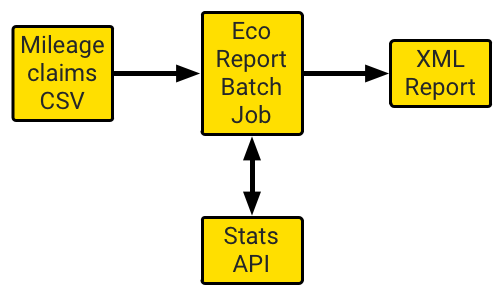
\includegraphics[width=\textwidth]{images/batch-job-overview-diagram}

\section*{Look at the code}

Take a look at the code that you've been given. There are plenty of files included that aren't being used yet, so while you work out how these classes relate to the diagram above, focus on:

\begin{itemize}
    \item \texttt{\ShoutyReportJob}
    \item \texttt{\ShoutyReportProcessor}
    \item \texttt{\ShoutyStatsServiceException}
    \item \texttt{\UnitTests}
    \item \texttt{\EndToEndTests}
    \item \texttt{\MileageClaim}
\end{itemize}

Find the tests that are included in the project. Don't run them yet.

\QandAbox{How would you describe these tests?}{3}

\QandAbox{Why do the end-to-end tests refer to a file called \texttt{report.xml}?}{3}

\section*{Run the tests}

\QandAbox{Did they all pass? If not, read the error report.}{3}

\begin{framed}
    "\emph{flaky} (adj.) - Not dependable nor trustworthy"
    \begin{flushright}
        \textit{JE Brown, Brown's Dictionary of Relationship Terms}
    \end{flushright}
\end{framed}

\QandAbox{Have you ever experienced a codebase that has \emph{flaky} tests? How did you cope?}{3}